% ===========================
% Chapters/1. Perfil.tex
% ===========================
\section{Perfil}

\subsection{Generalidades}

\subsubsection{Antecedentes del proyecto}
En Colombia hay 7,6 millones de personas de 60+ y la proporción seguirá creciendo hacia 2040. Una de cada tres sufre caídas cada año y, además, es frecuente el deterioro cognitivo leve asociado al sedentarismo. Esta combinación termina en pérdida de autonomía, mayor carga para las familias y presión sobre EPS/IPS. A nivel de sistema, las caídas representan costos cercanos al 1\% del PIB. 

En la práctica diaria se observan tres vacíos: (i) baja adherencia a rutinas tradicionales de ejercicio para equilibrio y reflejos, (ii) poco seguimiento objetivo en el hogar y (iii) ausencia de datos clínicos oportunos para ajustar tratamientos. Desde el punto de vista de mercado, \emph{salud digital} y \emph{tele-rehabilitación} muestran crecimiento sostenido en LatAm y existe espacio para soluciones accesibles orientadas a prevención.

A partir de este contexto, el proyecto \textbf{Equilibrado - Tecnología que te mantiene en pie} integra dispositivos de bajo costo, una aplicación móvil y un portal clínico para ofrecer sesiones lúdicas, seguimiento continuo y analítica útil para fisioterapeutas y aseguradoras. 

\textbf{Problema central del proyecto:} \emph{Falta de herramientas y procesos efectivos para la prevención de caídas en adultos mayores, con baja continuidad y escaso seguimiento de datos clínicos.}

\subsection{Concepción de la idea}

\subsubsection{Análisis del problema, la necesidad y la oportunidad; evaluación y valoración de ideas}
El punto de partida fue una matriz de ideas con fuentes de oportunidad (tendencias demográficas, adopción de interfaces de voz, evidencia de \textit{exergames} y propiocepción). Se evaluaron alternativas bajo cuatro perspectivas: personal (afinidad y capacidades), mercado (valor percibido, tamaño y estabilidad), recursos (equipo, tecnología, insumos, financiación) y legal (regulación, patentes y datos). 

La valoración (escala 1-5) arrojó como mejor desempeño tres propuestas: 
\begin{itemize}
    \item \textbf{SeniorGames} (\(\approx 3{,}51\)): juegos activos con sensores y niveles adaptativos.
    \item \textbf{Asistente virtual para la tercera edad} (\(\approx 3{,}34\)): recordatorio de medicación, chequeos de bienestar y acompañamiento.
    \item \textbf{ActivaVida - Dispositivo de equilibrio y reflejos} (\(\approx 3{,}33\)): hardware modular low-cost con métricas objetivas.
\end{itemize}

La decisión fue \textbf{fusionarlas} en una sola propuesta para capturar sinergias: hardware modular (IMU, disco, pads táctiles), \emph{exergames} que eleven adherencia, y un asistente digital (voz/notificaciones) que conecte a usuarios, cuidadores y fisios. La oportunidad se refuerza porque el modelo permite ingresos mixtos (venta/arriendo de kits + suscripción SaaS clínica) y genera datos clínicos accionables.

\paragraph{Propósito u objetivo general del proyecto.} \emph{Desarrollar un sistema integral y accesible que prevenga caídas y el deterioro cognitivo en adultos mayores, incremente la adherencia a los ejercicios, ofrezca monitoreo continuo y genere datos clínicos para una atención oportuna y de calidad.}

\subsubsection{Marco Lógico: análisis de grupos de interés}
La tabla resume actores, su rol y expectativas; se usará como insumo para el plan de relacionamiento y gestión de riesgos.

\begin{table}[H]
\centering
\renewcommand{\arraystretch}{1.2}
\begin{tabular}{p{2.8cm} p{2cm} p{2.5cm} p{3.5cm} p{4.8cm}}
\toprule
\textbf{Grupo} & \textbf{Rol} & \textbf{Tipo de participación} & \textbf{Intereses} & \textbf{Problemáticas / Mandatos \& recursos} \\
\midrule
Adultos mayores (60+) & Beneficiarios & Usan y retroalimentan & Seguridad, autonomía, sesiones sencillas y motivantes & Barreras digitales; comorbilidades; disponibilidad de tiempo. \\
Familias/cuidadores & Aliados & Acompañamiento y monitoreo & Tranquilidad, alertas oportunas, reportes claros & Carga de cuidado, coordinación con EPS/IPS. \\
Fisioterapeutas y clínicas & Socios técnicos & Diseño de protocolos y validación & Datos objetivos (sway, latencia), adherencia remota & Limitaciones de tiempo; integración con flujos clínicos. \\
EPS/aseguradoras & Pagadores & Contratos y evaluación & Reducción de siniestralidad y costos por caídas & Requisitos de evidencia y privacidad; interoperabilidad. \\
Gobiernos locales / sector público & Cooperantes & Articulación y soporte & Envejecimiento activo; programas preventivos & Normativa y tiempos de contratación pública. \\
Proveedores de hardware/software & Aliados & Suministro y soporte & Volumen estable y road-map claro & Certificaciones, calidad, continuidad de componentes. \\
Academia / redes geriátricas & Asesores & Investigación aplicada & Publicaciones, estudios de impacto & Tiempos de comités éticos y financiamiento. \\
Organizaciones de la sociedad civil & Difusores & Puente comunitario & Inclusión y actividades grupales & Aislamiento social; logística de sedes. \\
\bottomrule
\end{tabular}
\caption{Grupos de interés, roles y focos de gestión.}
\end{table}

\subsubsection{Marco Lógico: árbol de problemas (análisis)}
Del ejercicio se consolidó un árbol con \textit{causas indirectas} (demoras diagnósticas, falta de profesionales, saturación del sistema, baja cultura de ejercicio, escasa innovación), \textit{causas directas} (ineficacia de tratamientos, falta de monitoreo remoto, ausencia de programas lúdicos, poca tecnología adaptada), el \textbf{problema central} ya citado y sus \textit{efectos} (fracturas, costos, pérdida de autonomía, depresión, aislamiento y menor bienestar). 

\begin{figure}[H]\centering
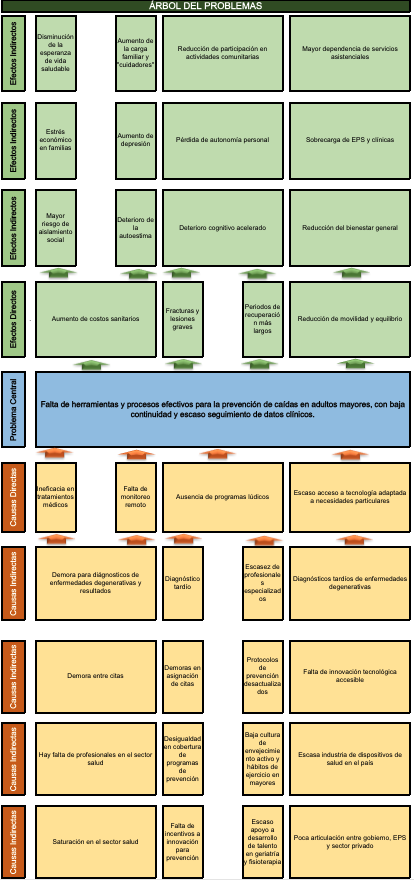
\includegraphics[width=.35\linewidth]{Figures/Arbol_Problemas/00_arbol_problemas_general.png}
\caption{Árbol de problemas — visión general.}
\end{figure}

\begin{figure}[H]\centering
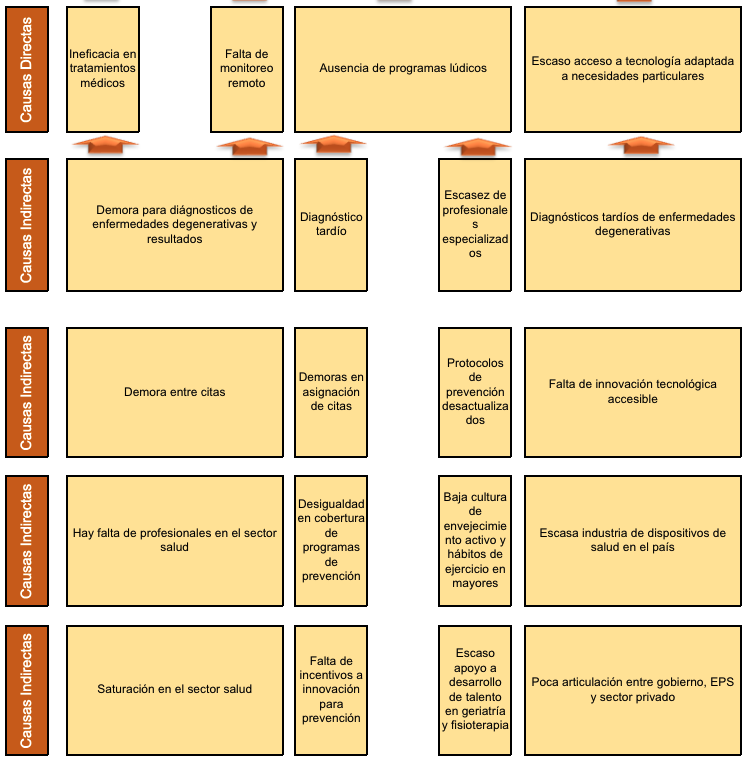
\includegraphics[width=.95\linewidth]{Figures/Arbol_Problemas/01_causas_directas_indirectas.png}
\caption{Detalle de \emph{Causas}: indirectas y directas.}
\end{figure}

\begin{figure}[H]\centering
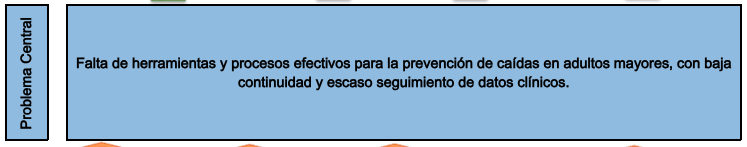
\includegraphics[width=.95\linewidth]{Figures/Arbol_Problemas/02_problema_central.png}
\caption{Problema central seleccionado.}
\end{figure}

\begin{figure}[H]\centering
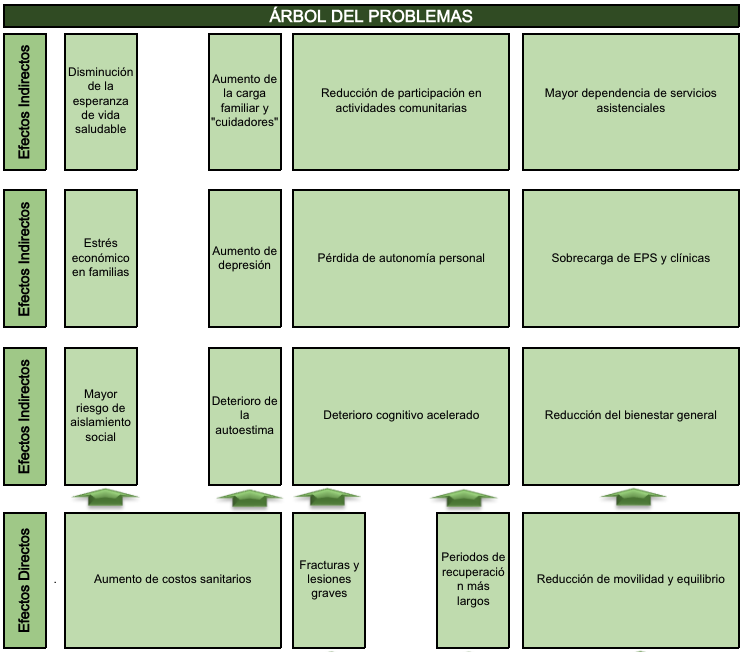
\includegraphics[width=.95\linewidth]{Figures/Arbol_Problemas/03_efectos_directos_indirectos.png}
\caption{Detalle de \emph{Efectos}: directos e indirectos.}
\end{figure}

\subsubsection{Marco Lógico: árbol de objetivos (análisis)}
El árbol de objetivos traduce cada causa en un medio y cada efecto en un fin. La \textbf{solución focal} se mantiene: \emph{sistema integral y accesible} que combina dispositivos lúdicos, app y analítica. Los objetivos específicos se enfocan en: (i) aumentar adherencia con gamificación y sesiones guiadas, (ii) habilitar monitoreo domiciliario y alertas, (iii) entregar reportes clínicos estandarizados para fisios/EPS y (iv) ampliar la cobertura mediante un modelo asequible.

\begin{figure}[H]\centering
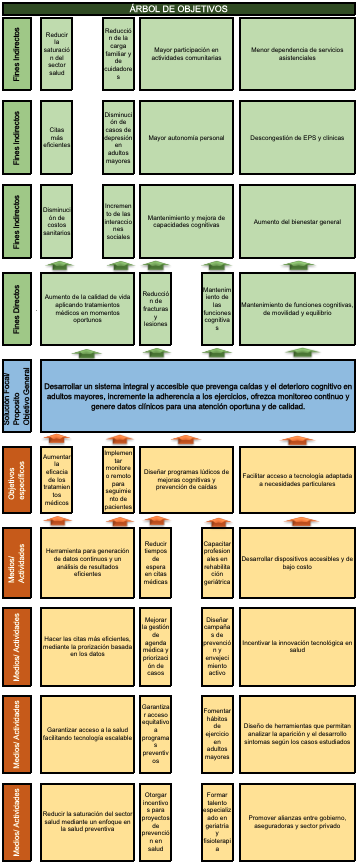
\includegraphics[width=.35\linewidth]{Figures/Arbol_Objetivos/00_arbol_objetivos_general.png}
\caption{Árbol de objetivos — visión general.}
\end{figure}

\begin{figure}[H]\centering
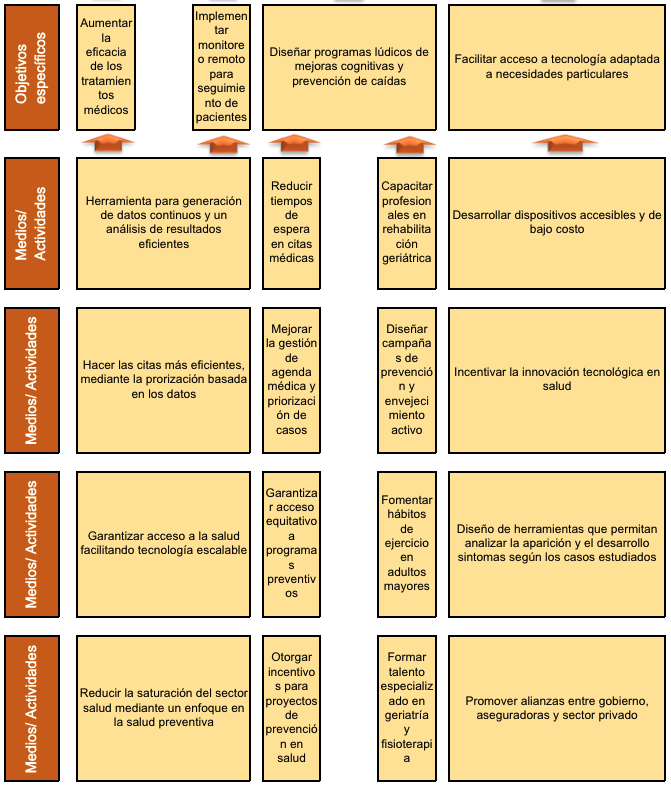
\includegraphics[width=.95\linewidth]{Figures/Arbol_Objetivos/01_medios_y_objetivos_especificos.png}
\caption{Medios/actividades y objetivos específicos.}
\end{figure}

\begin{figure}[H]\centering
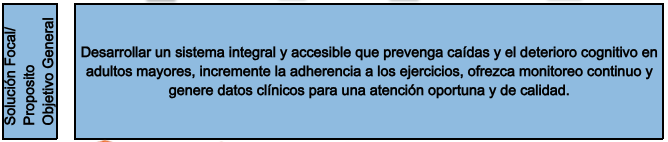
\includegraphics[width=.95\linewidth]{Figures/Arbol_Objetivos/02_solucion_focal_proposito.png}
\caption{Solución focal / Propósito u Objetivo General.}
\end{figure}

\begin{figure}[H]\centering
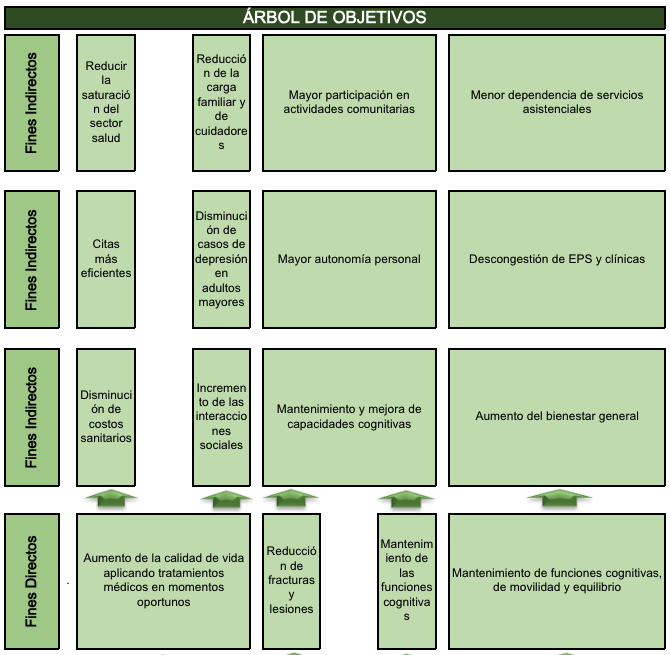
\includegraphics[width=.95\linewidth]{Figures/Arbol_Objetivos/03_fines_directos_indirectos.png}
\caption{Fines directos e indirectos.}
\end{figure}

\subsubsection{Marco Lógico: selección de la estrategia}
Con base en el análisis anterior, la estrategia priorizada es \textbf{Device-as-a-Service (DaaS)} con tres capas:
\begin{enumerate}
    \item \textbf{Dispositivos modulares} de bajo costo (banda IMU, disco, pads) conectados por BLE.
    \item \textbf{App} (React~Native) con \emph{exergames}, asistente de voz/notificaciones y seguimiento.
    \item \textbf{Portal clínico} (SaaS) con dashboards, reportes y APIs para EPS/IPS.
\end{enumerate}

\textbf{Justificación estratégica:}
\begin{itemize}
    \item \textit{Valor al usuario}: sesiones entretenidas que aumentan la práctica diaria y reducen riesgo.
    \item \textit{Valor al sistema de salud}: datos objetivos para ajustar planes, priorizar casos y prevenir eventos.
    \item \textit{Modelo de ingresos}: venta/arriendo de kits (margen meta 40\%) + suscripción mensual (B2C y clínica) + servicios de analítica a pagadores.
    \item \textit{Ejecución}: pilotos con 2 clínicas/50 pacientes, certificación sanitaria clase~I, red de \emph{Embajadores Senior}, alianzas con EPS y municipios.
\end{itemize}

\textbf{Indicadores guía}: reducción del 15\% en caídas, mejora del 20\% en tiempos de reacción y memoria funcional; 10.000 usuarios activos y 50 clínicas aliadas en 24 meses; retención 30-días \(\geq 60\%\).
